\title{Basic Lessons on Computer Olympiad: Logic and Math}
\date{\today}
\author{Azzam L. H.}
\maketitle
\renewcommand*\contentsname{Daftar Isi}

\begin{remark*}
    Mayoritas materi matematika disini diambil dari modul basic untuk OSN-K Matematika. Singkatan seperti OSK mengacu pada OSN-K Matematika sedangkan OSK Komputer baru mengacu pada OSN-K bidang informatika. Tetapi tenang saja, seluruh materi disini sesuai dengan silabus dan dasar-dasar materi yang dibutuhkan.
\end{remark*}
\tableofcontents

\newpage
\section{Logika Dasar}
\section{Common Math Mistakes}

\begin{enumerate}
    \item $\dfrac{n}{0} \neq \infty$ tetapi \textbf{seharusnya} $\dfrac{n}{0} = \text{tak terdefinisi}$ dimana $n \neq 0$.\\
    Kecuali kalau pakai limit, baru benar, yaitu $\lim_{x \rightarrow 0^+} \dfrac{n}{x} = \infty$ dan $\lim_{x \rightarrow 0^-} \dfrac{n}{x} = -\infty$
    \item Seharusnya $\dfrac{0}{0} = \textbf{tak tentu}$.
    \item $\pi$ (\textbf{pi}) itu \textbf{dibaca "PI"} bukan dibaca "FI". 
    \item Kalau $\varphi$ (\textbf{phi}) baru dibaca \textbf{"FI"}.
    \item $\sqrt{x} \ge 0$ dengan $x \ge 0$. Jadi, hasil dari $\sqrt{(-x)^2}=|x|$ jadinya $\sqrt{(-2)^2}=2$.
\end{enumerate}
\section{Logika Dasar}
\begin{enumerate}
    \item $A \land B$ dibaca $A$ dan $B$.
    \item $A \lor B$ dibaca $A$ atau $B$.
    \item $A \equiv B$ dibaca $A$ ekuivalen $B$ (untuk logika).
    \item $\exists x$ dibaca ada $x$ atau terdapat $x$.
    \item $\forall x$ dibaca untuk semua $x$.
    \item $A \implies B$ dibaca
    \begin{enumerate}
        \item $A$ hanya jika $B$,
        \item $B$ jika $A$,
        \item $A$ mengimplikasikan $B$,
        \item $A$ menyebabkan $B$,
        \item jika $A$ maka $B$.
    \end{enumerate}
    \item $A \Longleftarrow B$ dibaca $A$ jika $B$ (kebalikannya $\implies$).
    \item $A \iff B$ dibaca $A$ jika dan hanya jika $B$. Definisinya adalah $A \iff B \equiv (A \implies B) \land (A \Longleftarrow B)$.
\end{enumerate}
Apa bedanya $A \implies B$ dan $A \iff B$? Kalau $A \implies B$ berarti agar pernyataan benar haruslah $B$ benar, $A$ bisa salah atau benar. Kalau $A \iff B$, agar pernyataan benar, haruslah $A$ dan $B$ sama-sama benar atau sama-sama salah. Contohnya:
\begin{itemize}
    \item Jika sekarang hujan, maka saya tidak pergi. (Baik sekarang hujan ataupun tidak hujan, bisa saja saya tidak pergi, jadi tidak pengaruh).
    \item Saya laki-laki jika dan hanya jika saya bukan perempuan.
        \item Saya tidak bernafas selamanya jika dan hanya jika saya tidak hidup.
\end{itemize}
\section{Himpunan}
Hanya review, harusnya sejak SMP sudah paham mengenai himpunan / \textit{set} :).

Misalkan $A$ dan $B$ adalah dua himpunan.
\begin{enumerate}
    \item $\phi$ atau $\{\}$ adalah himpunan kosong atau himpunan yang tidak mempunyai elemen.
    \item Banyak elemen dari $A$ dinotasikan dengan $|A|$ (dibaca "kardinalitas dari $A$") atau $n(A)$ .
    \item $x \in A$ dibaca $x$ elemen dari $A$.
    \item $A \subseteq B$ dibaca $A$ subset dari $B$ atau $A$ himpunan bagian dari $B$.
    \item $A \subset B$ dibaca $A$ adalah proper subset dari $B$. Bedanya dengan $\subseteq$?\\
    $\subset$ itu mirip $<$ dimana tidak mungkin $A \subset A$, tetapi $\subseteq$ itu mirip $\le$ karena mungkin $A \subseteq A$.
    \item $A \cup B$ dibaca $A$ union $B$ atau $A$ gabung $B$.
    \item $A \cap B$ dibaca $A$ intersection $B$ atau $A$ irisan $B$.
    \item $A^c$ atau $A'$ dibaca $A$ komplemen.
    \item $|A \cup B| = |A|+|B|-|A \cap B|$.
\end{enumerate}
	
\subsection{Himpunan Bilangan-bilangan}
\begin{figure}[h]
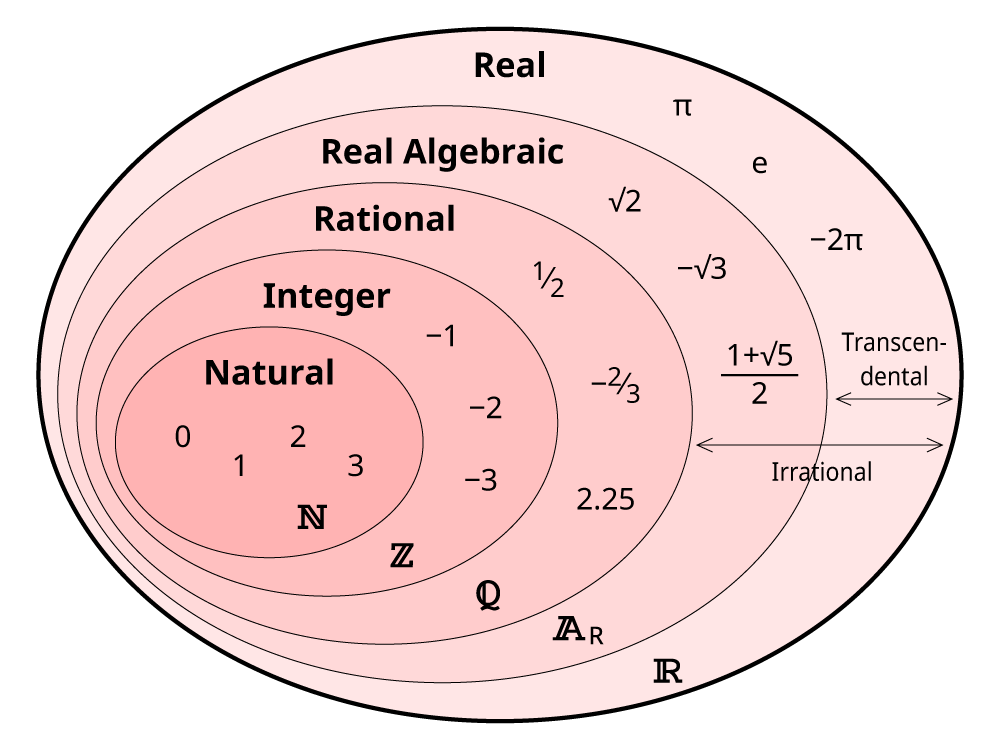
\includegraphics[width=\textwidth/2]{High/numbers set.png}
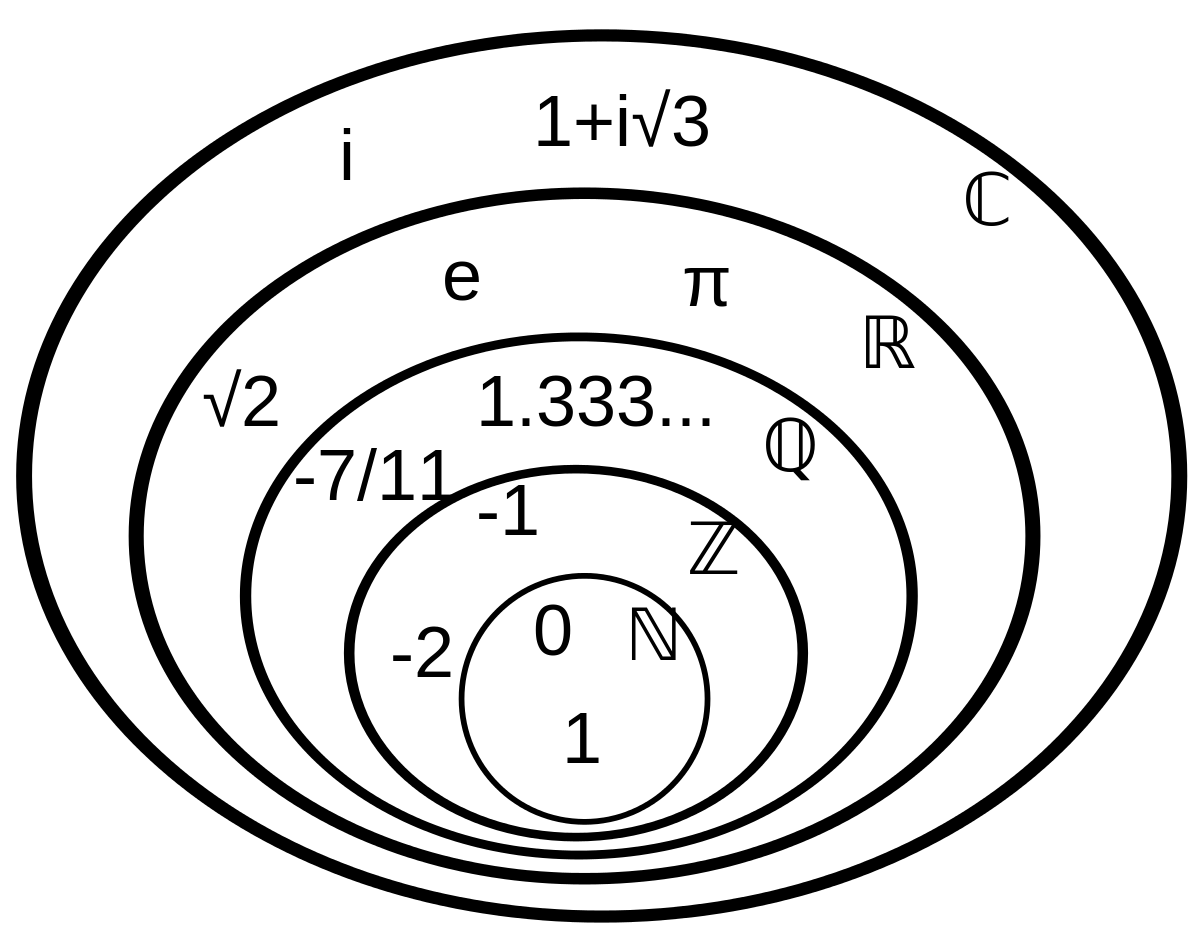
\includegraphics[width=\textwidth/2]{High/compset.png}
\caption{dari: https://thinkzone.wlonk.com/Numbers/RealSet\_w1000.png}
\caption{dan https://en.wikipedia.org/wiki/Number}
\end{figure}

\begin{enumerate}
\item $\NN$ adalah himpunan bilangan asli (Natural Numbers) $\{1,2,3,\dots\}$. Di beberapa negara Eropa dan beberapa negara lain, himpunan bilangan asli adalah $\{0,1,2,\dots\}$.
\item $\ZZ$ adalah himpunan bilangan bulat $\ZZ=\{\dots,-2,-1,0,1,2,\dots\}$.
\item $\QQ$ adalah himpunan bilangan rasional, dengan definisi $\QQ=\{\dfrac{a}{b}\mid a\in \ZZ, b\in\ZZ^+\}$.
\item $\RR$ adalah himpunan bilangan real, semua bilangan yang ada di dunia nyata, termasuk bilangan irasional seperti $\sqrt{2}$ dan rasional.
\item $\CC$ adalah himpunan bilangan kompleks dengan definisi\\ $\CC = \{a+bi \mid a,b \in \RR \text{ dan }i=\sqrt{-1}\}$.
\item Definisikan pula $\ZZ^+$ sebagai himpunan bialangan bulat positif. Aturan yang sama juga berlaku: $\RR^+, \QQ^+$.
\end{enumerate}

\section{Aljabar}
\subsection{Pemfaktoran dan Penguraian}
Tips: Jangan dihafal secara sengaja, tetapi banyak-banyaklah latihan soal, nanti hafal sendiri :D.
	
	Untuk $x,y,z \in \CC$.

        \subsubsection{\textit{Basic} yang paling sering muncul}
        \begin{enumerate}
            \item $x^2-y^2 = (x+y)(x-y)$.
	    \item $(x+y)^2 = x^2+2xy+y^2$.
	    \item $(x-y)^2 = x^2-2xy+y^2$.
            \item $(x+y)^3 = x^3+y^3+3xy(x+y) = x^3+3x^2y+3xy^2+y^3$. 
	    \item $(x-y)^3 = x^3-y^3+3xy(x-y) = x^3-3x^2y+3xy^2-y^3$. 
	    \item $x^3-y^3 = (x-y)(x^2+xy+y^2)$.
	    \item $x^3+y^3 = (x+y)(x^2-xy+y^2)$.
	    \item $x^n-y^n = (x-y)(x^{n-1}+x^{n-2}y+x^{n-3}y^2+\dots+xy^{n-2}+y^{n-1})$ untuk $n \in \NN$.
	    \item $x^n+y^n = (x+y)(x^{n-1}-x^{n-2}y+x^{n-3}y^2-\dots+xy^{n-2}+y^{n-1})$ untuk $n$ bilangan asli \textbf{ganjil}.
        \end{enumerate}

        \subsubsection{Lebih \textit{Advanced}}
	\begin{enumerate}
	    \item $(x+y+z)^2 = x^2+y^2+z^2+2xy+2yz+2zx$.
	    \item $x^2+y^2+z^2+xy+yz+zx = \frac12(x+y)^2+\frac12(y+z)^2+\frac12(z+x)^2$.
	    \item $x^2+y^2+z^2-xy-yz-zx = \frac12(x-y)^2+\frac12(y-z)^2+\frac12(z-x)^2$.
	    \item $x^3+y^3+z^3-3xyz = (x+y+z)(x^2+y^2+z^2-xy-yz-zx)$.
	    \item $(x+1)(y+1)(z+1)=xyz+xy+yz+zx+x+y+z+1$.
	    \item (Identitas Sophie Germain) $x^4+4y^4=(x^2+2xy+2y^2)(x^2-2xy+2y^2)$.
	    \item (Ekspansi Binomial) $(x+y)^n = {n \choose 0}x^ny^0 + {n \choose 1}x^{n-1}y^1+{n \choose 2}x^{n-2}y^2 + \dots + {n \choose n}x^0y^n$.
	    \item (Fermat Two Square Identity / Brahmagupta-Fibonacci Identity)\\
        $(a^2+b^2)(c^2+d^2)=(bc+ad)^2+(bd-ac)^2$ untuk $a,b,c,d \in \RR$.
	\end{enumerate}

 \subsection{Latihan Soal Pemfaktoran dan Manipulasi Aljabar}
\begin{enumerate}
    \item  Nilai dari $\sqrt{5050^2-4950^2}$ adalah \dots

    \item (OSP 2008) Jika $0 < b < a$ dan $a^2+b^2=6ab$, maka nilai $\dfrac{a+b}{a-b}=\dots$
    
    \item Jika $x > 0$ dan $x + \dfrac{1}{x} =  5$, maka nilai $x^3+\dfrac{1}{x^3}$ adalah \dots
    
    \item (OSK 2017) Diketahui $x-y=10$ dan $xy=10$. Nilai $x^4+y^4$ adalah \dots
    
    \item (OSK 2018) Diketahui $x$ dan $y$ bilangan prima dengan $x < y$, dan $x^3+y^3+2018=30y^2-300y+3018$. Nilai $x$ yang memenuhi adalah \dots
    
    \item Jika $a+b+c=0$ untuk suatu bilangan riil $a,b,c$, buktikan bahwa $a^3+b^3+c^3=3abc$.
    
    \item Jika $x=2021^3-2019^3$, maka nilai $\sqrt{\dfrac{x-2}{6}}$ adalah \dots

    \item (AIME 1987)
    Tentukan nilai sederhana dari $\dfrac{(10^4+324)(22^4+324)(34^4+324)(46^4+324)(58^4+324)}{(4^4+324)(16^4+324)(28^4+324)(40^4+324)(52^4+324)}$

    \item (OSK 2017) Jika $\dfrac{(a-b)(c-d)}{(b-c)(d-a)}=-\dfrac{4}{7}$, maka nilai dari $\dfrac{(a-c)(b-d)}{(a-b)(c-d)}$ adalah \dots

    \item (OSK 2019) Diketahui $a+2b=1$, $b+2c=2$, dan $b \neq 0$. Jika $a+nb+2018c = 2019$ maka nilai $n$ adalah \dots

    \item (OSK 2019) Misalkan $a = 2\sqrt{2} - \sqrt{8-4\sqrt{2}}$ dan $b = 2\sqrt{2} + \sqrt{8-4\sqrt{2}}$. Jika $\dfrac{a}{b}+\dfrac{b}{a}=x+y\sqrt{2}$ dengan $x,y$ bulat, maka nilai $x+y$ adalah \dots

    \item (OSK 2015) Diketahui bilangan real positif $a$ dan $b$ memenuhi persamaan
    \begin{align*}
        a^4+a^2b^2+b^4=6 \text{ dan } a^2+ab+b^2=4
    \end{align*}
    Nilai dari $a + b$ adalah \ldots

    \item (OSK 2022) Diketahui $a,b,c,d$ bilangan real positif yang memenuhi $a>c$, $d>b$, dan 
    $$3a^2+3b^2=3c^2+3d^2=4ac+4bd.$$
    Nilai $\dfrac{12(ab+cd)}{ad+bc}=\dots$ 
\end{enumerate}
\subsection{Eksponen}
Untuk $a,b,c \in RR$
\begin{enumerate}
    \item $a^0=1$ untuk $a \neq 0$.
    \item $a^n =  \underbrace{a \cdot a \cdot \ldots \cdot a}_{n \text{ kali}}$ untuk $n \in \NN$.
    \item $a^b\cdot a^c=a^{b+c}$.
    \item $a^b\cdot c^b = (ac)^b$.
    \item $\dfrac{a^b}{a^c}=a^{b-c}$ untuk $a\neq 0$.
    \item $(a^b)^c=a^{bc}$.
    \item $a^{-b} = \dfrac{1}{a^b}$ untuk $a \neq 0$.
    \item $\sqrt[n]{a^b}=a^{\dfrac{b}{n}}$ untuk $n \in \ZZ_{\ge 2}$
\end{enumerate}
\subsection{Latihan Soal Eksponen}
\begin{enumerate}
    \item Carilah jumlah semua bilangan bulat positif $a$ yang memenuhi $a^{(a-1)^{(a-2)}}=a^{a^2-3a+2}$.
    
    \item Carilah jumlah seluruh solusi real $x$ yang memenuhi $(x^2+5x+5)^{x^2-10x+21}=1.$
    
    \item Jika $5^x=6^y=30^7$, berapakah nilai $\dfrac{xy}{x+y}$?
\end{enumerate}
\subsection{Barisan dan Deret}
Simpelnya, \textbf{barisan} adalah kumpulan bilangan $a_1,a_2,\dots,a_n$ (beberapa buku atau author memulai dari $a_1$ namun ada juga yang memulai dari $a_0$, kita pakai yang dari $a_1$) yang memenuhi properti atau pola tertentu, sedangkan \textbf{deret} adalah jumlah bilangan-bilangan barisan tadi yaitu $a_1+a_1+a_2+\dots+a_n$ untuk suatu bilangan bulat non-negatif $n$.

Barisan dan deret di atas adalah barisan dan deret terbatas. Bagaimana dengan barisan dan deret tak hingga? Observasi saja nilai $n$ yang sangat besar, atau secara formal observasi saat $n \rightarrow \infty.$

\textbf{Sekali lagi barisan (bilangan-bilangan) $\neq$ deret (jumlah).}

Untuk anak SMP (dan SMA) barisan dan deret paling familiar adalah barisan dan deret aritmatika serta geometri. Untuk tantangan lebih lanjut, silakan kerjakan latihan soal :p.

\subsubsection{Notasi Sigma dan Pi}
Jumlah dari suku-suku pada suatu barisan dinotasikan dengan huruf sigma kapital:
$$\sum_{i=k}^{j} a_i = a_k+a_{k+1}+\dots+a_j.$$
Perkalian dari suku-suku pada suatu barisan dinotasikan dengan huruf pi kapital:
$$\prod_{i=k}^{j} a_i = a_k \cdot a_{k+1}\cdot \ldots \cdot a_j.$$

Ada juga $cyc$ sebagai notasi siklis dan $sym$ sebagai notasi simetris.

Misalkan kita akan mengevaluasi jumlah siklis dan simetris dari $a,b,c$.

Penjumlahan bersifat \textbf{siklis} apabila setiap suku tersebut dapat diperoleh dengan "menggeser" secara siklis atau "memutar" suku lainnya.
Contoh: $$\sum_{cyc} a = a+b+c$$
     $$\sum_{cyc} ab = ab+ bc + ca$$
Sedikit mirip dengan penjumlahan siklis, suatu penjumlahan bersifat \textbf{simetris} apabila setiap suku dapat diperoleh dari permutasi $n$ variabel dari suku-suku lainnya pada penjumlahan. Contoh: 
    $$\sum_{sym} a = a+b+c$$
    $$\sum_{sym} ab = ab+ ac + ba + bc + ca + cb$$
\subsubsection{Barisan dan Deret Aritmatika}
Barisan aritmatika in a nutshell: $a,a+b,a+2b,\dots$ dimana setiap \textbf{suku ke-$n$} dari barisan tersebut adalah $$a_n=a+(n-1)b$$ untuk suatu bilangan asli $n$ dan bilangan \textbf{real} $a,b$.

Lalu, \textbf{rumus deret}nya atau jumlah $n$ suku pertama barisan tersebut adalah (coba buktikan rumus ini) $$S_n = a_1+a_2+\dots+a_n=a+(a+b)+(a+2b)+\dots+(a+(n-1)b)=\dfrac{n}{2}(2a+(n-1)b).$$
\subsubsection{Barisan dan Deret Geometri}
 Barisan geometri in a nutshell: $a,ar,ar^2,\dots$ dimana setiap \textbf{suku ke-$n$} dari barisan tersebut adalah $$a_n=ar^{n-1}$$ untuk suatu bilangan asli $n$ dan bilangan \textbf{real} $a$ dan $r \neq 0$.

Lalu, \textbf{rumus deret}nya atau jumlah $n$ suku pertama barisan tersebut adalah (coba buktikan rumus ini) $$S_n = a_1+a_2+\dots+a_n=a+ar+ar^2+\dots+ar^{n-1}=\dfrac{a(1-r^n)}{1-r}.$$
Perhatikan jika $-1 < r < 1$ maka saat $n \rightarrow \infty$ rumus deret tak hingganya menjadi (why?) $$S_\infty =  \dfrac{a}{1-r}.$$

\subsection{Latihan Soal Barisan dan Deret}
\begin{enumerate}
\item (OSK 2006) Diketahui $a+(a+1)+(a+2)+\dots+50=1139$. Jika $a$ bilangan real positif, maka $a=\dots$

\item (AIME 1984) Barisan $a_1,a_2,\dots,a_{98}$ memenuhi $a_{n+1}=a_n+1$ untuk $n=1,2,\dots,97$ dan mempunyai jumlah sama dengan $137$. Tentukan nilai dari $a_2+a_4+a_6+\dots+a_{98}$.

\item (AIME 2003) Diketahui $0<a<b<c<d$ adalah bilangan bulat dimana $a,b,c$ membentuk barisan aritmatika sedangkan $b,c,d$ membentuk barisan geometri. Jika $d-a=30$ maka tentukan nilai dari $a+b+c+d$.

\item (OSK 2009) Bilangan bulat positif terkecil $n$ dengan $n> 2009$ sehingga $$\sqrt{\dfrac{1^3+2^3+3^3+\dots+n^3}{n}}$$
merupakan bilangan bulat adalah \dots

\item Tentukan nilai paling sederhana dari $\sqrt{2\sqrt{2\sqrt{2\sqrt{\dots}}}}$.

\item Tentukan nilai dari $\dfrac{1}{1\cdot2}+\dfrac{1}{2\cdot 3}+\dfrac{1}{3 \cdot 4}+\dots+\dfrac{1}{2020 \cdot 2021}.$

\item  Nilai paling sederhana dari $\left(1-\dfrac{1}{2^2}\right)\cdot\left(1-\dfrac{1}{3^2}\right)\cdot\left(1-\dfrac{1}{4^2}\right)\cdot\dots\cdot\left(1-\dfrac{1}{2021^2}\right)$ adalah \dots

\item Tentukan hasil dari jumlah $\dfrac{1}{\sqrt{1}+\sqrt{2}}+\dfrac{1}{\sqrt{2}+\sqrt{3}}+\dots+\dfrac{1}{\sqrt{99}+\sqrt{100}}.$

\item Nilai $x$ yang memenuhi persamaan
$$\sqrt{x\sqrt{x\sqrt{x\sqrt{\dots}}}}=\sqrt{4x+\sqrt{4x+\sqrt{4x+\sqrt{\dots}}}}$$
adalah \dots

\item Hitunglah nilai paling sederhana dari
$$6-\dfrac{5}{3+\dfrac{4}{3+\dfrac{4}{3+\dfrac{4}{3+\dfrac{4}{\dots}}}}}$$
\end{enumerate}
\subsection{Fungsi}
Fungsi $f : A \rightarrow B$ adalah suatu pemetaan dari $A$ ke $B$ dimana $A$ adalah domain dan $B$ adalah kodomain fungsi. Lebh lanjut, fungsi $f$ \textit{well-defined} jika untuk $\forall x \in A$ terdapat tepat satu (jadi ngga boleh ada dua) $y \in B$ sehingga $f(x)=y$. Himpunan seluruh $y$ hasil pemetaan fungsi tersebut dinamakan \textbf{range} fungsi $f$.

Tips-tips mengerjakan soal fungsi adalah (tergantung domainnya)
\begin{enumerate}
\item Substitusi $x=0$
\item Mengganti $x$ dengan $-x$
\item Mmebentuk suatu bentuk yang simetris (banyak-banyak latihan soal saja biar mengerti).
\end{enumerate}

\subsubsection{Fungsi Injektif (satu-satu)}
Definisi: Untuk setiap $x \in A$ ada tepat satu $y \in B$ sehingga $f(x)=y$. 
Catatan: Range dari fungsi $f$ tidak perlu mencover seluruh kodomain $B$.\\
Contoh: Dengan $f: \RR \rightarrow \RR$, $f(x)=x$, $f(x)=2x+3$, dll.\\ 
Contoh yang bukan fungsi injektif: Dengan $f(x)=x^2$ dari real ke real, misalkan $f(x)=4$, berarti $x=2$ dan $x=-2$, padahal biar injektif harusnya $x$ cuma satu aja.

\subsubsection{Fungsi Surjektif (Fungsi Onto)}
Definisi: Untuk setiap $y \in B$ terdapat $x \in A$ sehingga $f(x)=y$. 
Catatan: Dapat dikatakan range fungsi tersebut adalah kodomainnya juga (untuk sebagian besar kasus) atau dengan kata lain $f(x)$ "menyentuh" semua nilai yang mungkin di kodomainnya. \\
Contoh: $f(x)=x$, $f(x)=x^3$, dll.\\
Contoh yang bukan fungsi surjektif: $f(x)=x^4$ dari real ke real, perhatikan bahwa $f(x)$ harus "mengcover" semua nilai, namun adakah $x$ yang membuat $f(x)=-1$? Tidak ada bukan, berarti bukan fungsi surjektif.

\subsubsection{Fungsi Bijektif}
Fungsi yang injektif sekaligus surjektif.

\subsection{Komposisi Fungsi}
Simpelnya, fungsi di dalam fungsi. Untuk fungsi $f:A \rightarrow B$ dan $g:B \rightarrow C$, komposisi fungsinya adalah
$$(g \circ f)(x) = g(f(x)).$$

\subsubsection{Invers Fungsi}
Simpelnya kebalikan fungsi. Invers dari fungsi $f: A \rightarrow B$ adalah fungsi $f^{-1} : B \rightarrow A$ dengan didefinisikan sebagai
$$f^{-1}(f(x))=x.$$
Dengan kata lain, kita punya $f(x)=y$ jika dan hanya jika $f^{-1}(y)=x$.

\subsection{Latihan Soal Fungsi}
\begin{enumerate}
       \item Jika $f:\RR-\{0\} \rightarrow \RR$ adalah fungsi yang memenuhi $f(x)+2f\left(\frac{1}{x}\right)=3x$ untuk setiap bilangan real $x \neq 0$, maka tentukan nilai $f(2021).$

\item (OSP 2004) Misalkan $f$ sebuah fungsi yang memenuhi $f(x)f(y)-f(xy)=x+y,$ untuk setiap bilangan bulat $x$ dan $y$. Berapakah nilai $f(2004)$?

\item (OSK 2011) Misalkan $f$ suatu fungsi yang memenuhi $f(xy) = \dfrac{f(x)}{y}$ untuk semua bilangan real positif $x$ dan $y$. Jika $f(100)=3$ maka $f(10)$ adalah \dots

\item (OSP 2009) Suatu fungsi $f:\ZZ \rightarrow \QQ$ mempunyai sifat $f(x+1)=\dfrac{1+f(x)}{1-f(x)}$ untuk setiap $x \in \ZZ$. Jika $f(2)=2$, maka nilai fungsi $f(2009)$ adalah \dots
\end{enumerate}

\section{Kombinatorika}
Notasikan $n!=n \times (n-1) \times (n-2) \times \dots \times 3 \times 2 \times 1$ (dibaca $n$ faktorial) dengan $1!=0!=1$.
\subsection{Aturan Pencacahan}
\subsection{Latihan Soal Pencacahan: Aturan Penjumlahan dan Perkalian}
\begin{enumerate}
    \item Misalkan Michie mempunyai 3 buah celana dan 4 buah baju. Berapa banyak cara Michie memilih celana dan baju yang akan dipakai ?

    \item Berapa banyak cara menyusun huruf-huruf R, A, J, I, N jika 
    \begin{enumerate}
        \item huruf pertama dimulai dari huruf hidup (vokal) 
        \item huruf pertama dimulai dari huruf mati (konsonan) 
    \end{enumerate}

    \item Sembilan orang siswa akan duduk pada 5 kursi sejajar. Ada berapa cara susunan mereka ? 
    
    \item Denny akan membentuk bilangan genap 3 angka yang angka-angkanya diambil dari 2, 3, 4, 5, 6, 7, 8. Berapa banyak bilangan yang dapat dibentuk jika : 
    \begin{enumerate}
        \item angka-angkanya boleh berulang 
        \item angka-angkanya tidak boleh berulang
    \end{enumerate}

    \item (OSK 2003) Ada berapa banyak bilangan 4-angka (digit) yang semua angkanya genap dan bukan merupakan kelipatan 2003 ?

    \item Sekumpulan orang duduk mengelilingi sebuah meja bundar. Diketahui ada 7 wanita dimana di sebelah kanan setiap wanita tersebut adalah wanita dan ada 12 wanita yang di sebelah kanan setiap wanita tersebut adalah pria. Diketahui pula bahwa 3 dari 4 pria di sebelah kanannya adalah wanita. Berapa orang yang duduk mengelilingi meja tersebut?

    \item (OSK 2015) Masing-masing kotak pada papan catur berukuran $3 \times 3$ dilabeli dengan satu angka yaitu 1, 2, atau 3. Banyaknya penomoran yang mungkin sehingga jumlah angka pada masing-masing baris dan masing-masing kolom habis dibagi 3 adalah \ldots
\end{enumerate}
\subsection{Permutasi}
Permutasi $k$ unsur dari $n$ unsur adalah (urutan diperhatikan)
$$_nP_k = P_k^n = \dfrac{n!}{(n-k)!}.$$
\subsection{Kombinasi}
Kombinasi $k$ unsur dari $n$ unsur adalah (urutan tak diperhatikan)
$${n \choose k}=_nC_k = C_k^n = \dfrac{n!}{k!(n-k)!}.$$
\subsection{Latihan Soal Kombinasi}
\begin{enumerate}   
    \item  Carilah banyaknya menempatkan 3 benteng (rooks) pada papan catur $5 \times 5$ sehingga tidak ada dua catur yang dalam posisi dapat saling menyerang.

    \item Carilah banyaknya kuadrupel terurut bilangan ganjil positif $(x_1, x_2, x_3, x_4)$ yang memenuhi $x_1 + x_2 + x_3 + x_4 = 98$.

    \item Perhatikan gambar berikut. 
    
    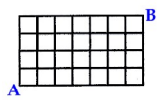
\includegraphics[width=0.2\linewidth]{Soal/Combinatorics/shortestPath.PNG} 
    
    Jika seseorang akan berjalan dari titik A ke titik B. Ada berapa banyak cara jalan terpendek yang dapat dipilihnya ?

    \item (OSK 2010) Banyaknya himpunan $X$ yang memenuhi 
    $$\{1,2,\dots,1000\} \subseteq X \subseteq \{1,2,\dots,2010\}.$$

    \item (OSP 2010) Bilangan asli enam digit $abcdef$ dengan $a > b > c \ge d > e > f$ ada sebanyak \dots
    
    \item (OSK 2017)
	Sebuah hotel mempunyai kamar bernomor 000 sampai dengan 999. Hotel tersebut menerapkan aturan aneh sebagai berikut: jika suatu kamar berisi tamu, dan sembarang dua digit nomor kamar tersebut dipertukarkan tempatnya, maka diperoleh nomor kamar yang sama atau nomor kamar yang tidak berisi tamu. Maksimal banyaknya kamar yang berisi tamu adalah \dots
\end{enumerate}
\subsection{Permutasi Siklis}
$n$ objek ditaruh mengelilingi lingkaran maka banyak cara menyusunnya adalah
$$P_{siklis} =\dfrac{n!}{n} = (n-1)!$$
\subsection{Prinsip Inklusi Eksklusi}
Prinsip Inklusi (memasukkan, dari kata inklusif) Eksklusi (mengeluarkan, khusus, dari kata eksklusif) atau yang sering disingkat PIE, pada dasarnya adalah konsep dari mengurangi "kelebihan hitung" atau menambahkan "kekurangan hitung". Contohnya adalah soal himpunan yang dinyatakan dalam rumus berikut
$$|A \cup B|=|A|+|B|-|A \cap B|.$$

Untuk tiga himpunan $A,B,C$ adalah
$$|A \cup B \cup C|=|A|+|B|+|C|-|A \cap B|-|A \cap C|-|B \cap C|+|A \cap B \cap C|.$$

dan seterusnya. Lebih lengkapnya boleh mengacu ke \href{https://brilliant.org/wiki/principle-of-inclusion-and-exclusion-pie/}{https://brilliant.org/wiki/principle-of-inclusion-and-exclusion-pie/}

\subsubsection{Derangement}
Teorema ini juga bisa disebut "teorema kado silang". Bunyi teorema ini:

Misalkan $n$ adalah bilangan bulat non-negatif. Kita sebut $!n$ atau $D_n$ sebagai derangement dari $n$ yaitu banyaknya permutasi $n$ elemen berbeda sedemikian sehingga tidak ada elemen yang menempati tempatnya semula.

\textbf{Versi yang tidak terlalu abstrak:} $!n$ adalah derangement dari $n$, dimana misalkan pada sebuah pesta ulang tahun, $n$ orang saling bertukar kado (awalnya semua orang mempunyai tepat satu kado) dimana setelah bertukar kado tidak ada orang yang mendapat kado dari dirinya sendiri. Banyak kemungkinan pertukaran kado ini adalah $!n$.

Rumus umum untuk menghitung derangement adalah
$$!n = n! \left(\dfrac{1}{0!}-\dfrac{1}{1!}+\dfrac{1}{2!}-\dfrac{1}{3!}+\dfrac{1}{4!}-\dfrac{1}{5!}+\dots+(-1)^n\dfrac{1}{n!}\right).$$
\subsection{Pigeon Hole Principle (PHP)}
Teorema yang dalam Bahasa Indonesia ini disebut dengan Teorema Sangkar Burung Merpati secara matematis berbunyi:
Jika ada $kn+1$ merpati dan $n$ sangkar, maka setidaknya ada satu sangkar yang berisi $k+1$ burung merpati.

Versi lebih simpelnya adalah: jika ada $n+1$ objek yang akan dibagi ke dalam $n$ buah kotak, maka setidaknya ada 1 kotak yang berisi 2 objek.

Contoh: \begin{itemize}
    \item Di dalam ruangan berisi 3 orang, pasti terdapat setidaknya 2 orang berjenis kelamin sama.
    \item Jika ada 367 orang di suatu sekolah, maka setidaknya ada dua orang diantara mereka yang tanggal lahirnya persis sama.
\end{itemize}
\subsection{Peluang}
Misalkan kita melempar sekeping koin, maka kegiatan ini disebut dengan percobaan. Hasil percobaan yang didapat biasanya adalah munculnya sisi gambar, $G$, atau munculnya sisi tulisan, $T$. Ruang contoh atau ruang sampel adalah himpunan dari \textbf{semua hasil percobaan yang mungkin} biasanya dilambangkan dengan $S$, yang dalam teori himpunan disebut dengan himpunan semesta. Pada percobaan melempar koin, ruang sampelnya adalah $\{G, T\}$ sedangkan pada percobaan melempar satu buah dadu, ruang sampelnya adalah $\{1, 2, 3, 4, 5, 6\}$. Jika $\{G, T\}$ adalah ruang sampel, maka anggota-anggota dari ruang sampel tersebut disebut titik contoh. Titik contoh dari $\{G, T\}$ adalah $G$ dan $T$. Pada percobaan melempar satu buah dadu seimbang, titik sampel yang didapat ada 6 yaitu 1, 2, 3, 4, 5, 6 sedangkan jika melempar dua buah dadu akan didapat 36 buah titik contoh, yaitu $(1, 1), (1, 2), (1, 3), \dots , (6, 6)$. 

\subsubsection{Formula Penghitungan Peluang}
Secara mudahnya, enghitung peluang bisa dengan pendekatan frekuensi, yaitu suatu percobaan yang dilakukan sebanyak $n$ kali, ternyata kejadian $A$ munculnya sebanyak $k$ kali, maka frekuensi nisbi/relatif kejadian $A$ sama dengan 
$$p(A)=\dfrac{k}{n}$$
Kalau $n$ semakin besar dan menuju tak terhingga maka nilai $p(A)$ akan cenderung konstan mendekati suatu nilai tertentu yang disebut dengan peluang munculnya kejadian $A$.

\subsection{Stars and Bars}
Banyaknya solusi bulat non-negatif $(x_1,x_2,\dots,x_k)$ dari sistem persamaan $x_1+x_2+\dots+x_k=n$ adalah
$${n+k-1 \choose k-1}.$$
Banyaknya solusi bulat positif $(x_1,x_2,\dots,x_k)$ dari sistem persamaan $x_1+x_2+\dots+x_k=n$ adalah
$${n-1 \choose k-1}.$$

\subsection{Latihan Soal Stars and Bars}
\begin{enumerate}
    \item Carilah banyaknya kuadrupel terurut bilangan ganjil positif $(x_1, x_2, x_3, x_4)$ yang memenuhi $x_1 + x_2 + x_3 + x_4 = 98$.
\end{enumerate}
\subsection{Identitas Kombinatorika}
\begin{enumerate}
    \item  ${n \choose k} = {n \choose n-k}$ dengan $k,n \in \NN_0$ dan $k \le n$.
    \item (Identitas Pascal) Untuk $n,k \in \NN_0$ berlaku ${n \choose k} + {n \choose k+1} = {n+1 \choose k+1}$
    \item (Hockey Stick Identity) Untuk $n,r\in\mathbb{N}, n>r,\sum^n_{i=r}{i\choose r}={n+1\choose r+1}$.
    \item Untuk $n,k \in \NN_0$ berlaku ${n \choose 0}+{n \choose 1} + \dots + {n \choose n} = 2^{n}$.
    \item Untuk $n,k \in \NN_0$ berlaku ${n \choose 0}+{n \choose 2} + \dots + {n \choose 2\floor{\frac{n}{2}}} = 2^{n-1}$.
    \item (Vandermonde's Identity)  $\sum_{k=0}^r\binom mk\binom n{r-k}=\binom{m+n}r$
\end{enumerate}

\subsection{Latihan Soal Identitas Kombinatorika}
\begin{enumerate}
    \item (AIME II 2000) Given that
            $\frac 1{2!17!}+\frac 1{3!16!}+\frac 1{4!15!}+\frac 1{5!14!}+\frac 1{6!13!}+\frac 1{7!12!}+\frac 1{8!11!}+\frac 1{9!10!}=\frac N{1!18!}$
            find the greatest integer that is less than $\frac N{100}$. 

        \item (AIME 1986) The polynomial $1-x+x^2-x^3+\cdots+x^{16}-x^{17}$ may be written in the form $a_0+a_1y+a_2y^2+\cdots +a_{16}y^{16}+a_{17}y^{17}$, where $y=x+1$ and the $a_i$'s are constants. Find the value of $a_2$.

        \item (AMC 10A 2016) For some particular value of $N$, when $(a+b+c+d+1)^N$ is expanded and like terms are combined, the resulting expression contains exactly $1001$ terms that include all four variables $a, b,c,$ and $d$, each to some positive power. What is $N$?
\end{enumerate}
\subsection{Binomial Newton}
Binomial Newton atau ekspansi/penjabaran binomial berfokus pada nilai koefisien setiap suku hasil penjabaran $(a+b)^n$.
$$(a+b)^n = {n \choose 0} a^nb^0 + {n \choose 1} a^{n-1}b^1+ \dots +{n \choose n}a^0b^n$$
\subsection{Latihan Soal Ekspansi Binomial Newton}
\begin{enumerate}
    \item Carilah koefisien $x^4$ dari penjabaran $(x+1)^9$

\item (OSK 2013) Koefisien $x^{2013}$ pada ekspansi
$$(1+x)^{4026}+x(1+x)^{4025}+x^2(1+x)^{4024}+\dots x^{2013}(1+x)^{2013}$$
adalah \dots

\item Jika $S=(\sqrt{71}+1)^{71}-(\sqrt{71}-1)^{71}$ adalah bilangan bulat, carilah digit terakhir dari $S$
\end{enumerate}

\subsection{Relasi Rekurensi}
Sering disebut dengan rekursif. Intinya adalah sebuah persamaan yang melibatkan barisan $a_1, a_2, \dots , a_n$ dimana untuk mendapatkan nilai $a_k$ membutuhkan suku-suku sebelumnya $a_{k-1}, a_{k-2}, \dots,$ atau $a_1$. 

Contoh paling terkenal dari persamaan rekursif adalah bilangan Fibonacci $0,1,1,2,3,5,8,13,21,\dots$ yang secara matematis didefinisikan sebagai berikut.
\begin{align*}
    F_0 &= 0, F_1 = 1\\
    F_n &= F_{n-1}+F_{n-2} \text{ untuk } n \ge 2
\end{align*}

atau yang lebih terkenal di ranah \textit{Computer Science} adalah permasalahan \textit{Tower of Hanoi} dengan persamaan rekursifnya didefinisikan sebagai berikut.
\begin{align*}
    T_1 &= 1 \\
    T_n &= 2T_{n-1}+1
\end{align*}

Untuk menyelesaikan soal relasi rekurensi, butuh manipulasi aljabar yang mumpuni sehingga tidak ada pendekatan eksplisit selain menggunakan persamaan karakteristik atau fungsi pembangkit (tidak dibahas disini) yang dijamin berhasil.

\subsubsection{Persamaan Karakteristik untuk Relasi Rekurensi Linear}
Persamaan karakteristik berikut berlaku untuk persamaan rekursif yang linear. Persamaan karakteristik berikut berguna untuk mengubah relasi rekurensi menjadi iteratif, atau persamaan berbentuk implisit. (Jadi, untuk persamaan yang bukan linear, sebagai contoh $a_n = a_{n-1}^2 + a_{n-2}$ tidak bisa dijamin selesai dengan persamaan karakteristik yang disajikan berikut).
Untuk persamaan rekursif
$$a_n = c_1a_{n-1}+c_2a_{n-2}+\dots+c_da_{n-d}$$
mempunyai persamaan karakteristik
$$x^d-c_1x^{d-1}-c_2x^{d-2}-\dots-c_dx^0=0$$

Sebagai contoh, rumus rekursif dari barisan Fibonacci di atas dapat diselesaikan menjadi 
$$x^{n}-x^{n-1}-x^{n-2}=0 \implies x^2-x-1=0$$
yang mempunyai dua akar, yaitu $x_1 = \dfrac{1+\sqrt{5}}{2}=\phi$ dan $x_2 = \dfrac{1-\sqrt{5}}{2}=1-\phi$ dimana $\phi$ adalah \textit{Golden Ratio}. Sadari bahwa setiap suku di barisan Fibonacci tersebut berbentuk $F_n = c_1x_1^n + c_2x_2^n$ (buktikan). Dengan substitusi $x_1$ dan $x_2$ serta pemilihan suku dari barisan Fibonacci (misal suku pertama dan kedua) maka akan ditemukan nilai $c_1$ dan $c_2$ sehingga pada akhirnya kita punya
$$F_n=\dfrac{\phi^n-(1-\phi)^n}{\sqrt{5}}$$


\section{Teori Bilangan}
\subsection{Paritas Penjumlahan dan Perkalian antara Dua Bilangan}
Paritas dalam konteks ini adalaha "genap-ganjil" nya suatu bilangan.
    \begin{enumerate}
        \item Bilangan Ganjil $\pm$ Bilangan Ganjil = Bilangan Genap 
        \item Bilangan Genap $\pm$ Bilangan Ganjil = Bilangan Ganjil 
        \item Bilangan Genap $\pm$ Bilangan Genap = Bilangan Genap 
        \item Bilangan Ganjil $\times$ Bilangan Ganjil = Bilangan Ganjil 
        \item Bilangan Ganjil $\times$ Bilangan Genap = Bilangan Genap 
        \item Bilangan Genap $\times$ Bilangan Genap = Bilangan Genap
    \end{enumerate}
    Dari sifat-sifat perkalian dua bilangan akan didapat bahwa bilangan genap tidak mungkin membagi bilangan ganjil sedangkan bilangan ganjil mungkin membagi bilangan genap. 


    
\subsection{Keterbagian}
    Untuk bilangan bulat $a \neq 0$ serta bilangan bulat $b,c,x$ dan $y$, notasikan $a \mid b$ sebagai $a$ membagi $b$. Lalu, $a$ dan $b$ relatif prima atau $a$ dan $b$ koprima (coprime) jika dan hanya jika $FPB(a,b)=1$.
    \begin{enumerate}
        \item Kita dapat menyatakan semua bilangan bulat $c = pq+r$ untuk suatu bilangan bulat $q$ dimana $0 \le r < q$. Jadi, saat $c$ dibagi $p$, maka hasil baginya adalah $q$ dan sisa baginya adalah $r$.
        \item Terdapat suatu bilangan bulat $x$ dimana $a \mid b \iff b=ax$.
        \item $a \mid a$.
        \item $a \mid 0$.
        \item $1 \mid a$.
        \item $a \mid b \implies a \mid bc$.
        \item Untuk $a,b \neq 0$ maka $ab \mid c \implies a \mid c \text{ dan } b \mid c$.
        \item $a \mid b \text{ dan } b \mid c \implies a \mid c$.
        \item $a \mid b \text{ dan } a \mid c \implies a \mid bx + cy$.
        \item $a \mid b \text{ dan } a \mid c \implies a \mid b+c$.
        \item $a \mid b \text{ dan } a \mid c \implies a \mid b-c$.
        \item Untuk $x \neq 0$ maka $a \mid b \iff xa \mid xb$.
        \item $a \mid b$ dan $b \neq 0$ maka $|a| \le |b|$.
        \item $a \mid bc$ dan $FPB(a,b)=1$ maka $a\mid c$.
    \end{enumerate}


    
\subsection{Aritmatika Modular}
    Untuk suatu bilangan asli $m$ dan bilangan bulat $a,b,c$ dan $d$, notasikan $m\mid a-b \iff a \equiv b \mod m$ (dibaca $a$ kongruen $b$ modulo $m$). Simpelnya $a \equiv b \mod m$ adalah $a$ dibagi $m$ bersisa $b$. Contohnya $5 \equiv 2 \mod 3$. $13 \equiv 3 \mod 5$. $10 \equiv -2 \mod 12$.
    \begin{enumerate}
        \item $a \equiv a \mod m$.
        \item $a \equiv 0 \mod m \iff m\mid a$.
        \item $a \equiv b \mod m \iff b \equiv a \mod m$.
        \item $a \equiv b \mod m \text{ dan } b \equiv c \mod m \implies a \equiv c \mod m$.
        \item Jika $a \equiv b \mod m$ dan $d\mid m$ maka $a \equiv b \mod d$.
        \item Untuk semua bilangan asli $k$, $a \equiv b \mod m \iff a^k \equiv b^k \mod m$.
        \item $a \equiv b \mod m \text{ dan } c \equiv d \mod m \implies a+c \equiv b+d \mod m$.
        \item $a \equiv b \mod m \text{ dan } c \equiv d \mod m \implies a-c \equiv b-d \mod m$.
        \item $a \equiv b \mod m \text{ dan } c \equiv d \mod m \implies ac \equiv bd \mod m$.
        \item $\forall k\in \ZZ^+, (am+b)^k \equiv b^k \mod m$.
        \item Jika $ca \equiv cb \mod m$ dengan $FPB(c,m)=1$, maka $a \equiv b \mod m$.
    \end{enumerate}
    
    Catatan: Penggunaan sifat nomor 8 dapat dimodifikasi sehingga menjadi konsep \textbf{Chinese Remainder Theorem}.

\subsection{Latihan Soal Aritmatika Modular}
\begin{enumerate}    
    \item (AIME 1986) Tentukan bilangan asli $n$ terbesar sehingga $n+10 \mid n^3+100$.
    
    \item Tentukan digit satuan dari $7^{7^7}$.
    
    \item Jika $S=1!+2!+3!+\dots+2021!$, tentukan sisa $S$ saat dibagi 6.
    
    \item (OSK 2009) Sisa saat $10^{999999999}$ saat dibagi oleh 7 adalah \dots
    
    \item (OSK 2011) Bilangan asli terkecil $n>2011$ yang bersisa 1 jika dibagi $2,3,4,5,6,7,8,9,10$ adalah \dots.

    \item (OSK 2015) Bilangan $x$ adalah bilangan bulat positif terkecil yang membuat
    \[31^n + x \cdot 96^n\]
    merupakan kelipatan 2015 untuk setiap bilangan asli $n$. Nilai $x$ adalah \ldots
\end{enumerate}
\subsection{Uji habis dibagi}
    Trik yang suatu saat dapat membuat hidup anda bahagia :D. Semua rumus ini dapat dibuktikan dengan aritmatika modular.
    \begin{enumerate}
        \item Bilangan $x$ genap jika dan hanya jika digit terakhir $x$ genap.
        \item $3 \mid x$ jika dan hanya jika jumlah digit-digitnya habis dibagi $3$. Contohnya 2931 habis dibagi 3 karena $2+9+3+1=15$ habis dibagi 3.
        \item $9 \mid x$ jika dan hanya jika jumlah digit-digitnya habis dibagi $9$.
        \item $x$ habis dibagi 5 jika dan hanya jika digit terakhir $x$ adalah $0$ atau $5$.
        \item $x$ habis dibagi 11 jika dan hanya jika jumlah selang-seling (alternate sums) dari digit-digitnya habis dibagi 11. Contoh: 945351 habis dibagi 11 karena $9-4+5-3+5-1=11$ habis dibagi 11. 121 habis dibagi 11 karena $1-2+1=0$ habis dibagi 11.
    \end{enumerate}


    
\subsection{FPB dan KPK dua bilangan}
Secara matematis FPB (gcd - greatest common divisors) dan KPK (lcm - least common multiples) dari dua bilangan bulat positif $a$ dan $b$ 
didefinisikan sebagai:
$$FPB(a,b) = gcd(a,b) = p_1^{\min\{a_1,b_1\}}\cdot p_2^{\min\{a_2,b_2\}} \cdot \ldots \cdot p_n^{\min\{a_n,b_n\}}$$
$$KPK(a,b) = lcm(a,b) =p_1^{\max\{a_1,b_1\}}\cdot p_2^{\max\{a_2,b_2\}} \cdot \ldots \cdot p_n^{\max\{a_n,b_n\}}$$
dimana kedua bilangan tersebut dapat difaktorisasi prima menjadi
$a=p_1^{a_1}\cdot p_2^{a_2}\cdot \ldots \cdot p_n^{a_n}$ dan $b=p_1^{b_1}\cdot p_2^{b_2} \cdot \ldots \cdot p_n^{b_n}$, dengan $p_1,p_2,\dots,p_n$ adalah bilangan prima berbeda, serta $a_1,a_2,\dots,a_n,b_1,b_2,\dots,b_n$ adalah bilangan bulat non-negatif.

Dari definisi tersebut mudah dibuktikan bahwa
$$FPB(a,b) \cdot KPK(a,b) = ab.$$

Perlu dicatat, bahwa $a$ dan $b$ tidak boleh bernilai nol. Untuk $a,b$ yang bernilai negatif, didefinisikan $FPB(a,b) = FPB(|a|,|b|)$.

\subsubsection{Algoritma Euclid}
Pada dasarnya algoritma ini bertumpu pada sebuah teorema:
$$FPB(a,b) = FPB(a,b-a) = FPB(a-b,b)=FPB(a, b \mod a)$$

\subsection{Latihan Soal FPB dan KPK}
\begin{enumerate}
    \item (OSK 2011) Bilangan asli terkecil lebih dari 2011 yang bersisa 1 jika dibagi 2,3,4,5,6,7,8,9,10 adalah \dots
    
    \item (OSK 2009) Nilai dari $\sum_{k=1}^{2009} FPB(k,7)$ adalah \dots
    
    \item Banyaknya anggota himpunan himpunan 
    $$S = \{gcd(n^3+1,n^2+3n+9 \mid n \in Z\}$$
    adalah \dots
    
    \item (AIME 1998) Ada berapa banyak bilangan bulat positif $k$ sehingga $lcm(6^6,8^8,k)=12^{12}$?
    
    \item Jika $a,b$ adalah bilangan asli dan $c$ adalah bilangan bulat, buktikan bahwa $gcd(a,b)=gcd(a,b+ac).$
\end{enumerate}
\subsubsection{Algoritma Euclid}
Pada dasarnya algoritma ini bertumpu pada sebuah teorema:
$$FPB(a,b) = FPB(a,b-a) = FPB(a-b,b)=FPB(a, b \mod a)$$

\subsection{Fungsi yang Melibatkan Faktor Bilangan}
Misalkan $a$ dapat difaktorisasi prima seperti sebelumnya yaitu $a=p_1^{a_1}\cdot p_2^{a_2}\cdot \ldots \cdot p_n^{a_n}$.
\subsubsection{Banyaknya Faktor Positif}
Fungsi $d(a)$ didefinisikan sebagai banyaknya faktor atau pembagi positif dari $a$ dengan
$$d(a) = (a_1+1)(a_2+1)\cdot \ldots \cdot (a_n+1).$$

Contoh: Banyaknya faktor positif dari $12= 2^2 \cdot 3^1$ adalah $d(12)=(2+1)(1+1)=6$ dengan pembagi positifnya adalah $1,2,3,4,6,12$ (ada 6 faktor positif.)
\subsubsection{Jumlah Faktor Positif}
Fungsi $\sigma (a)$ didefinisikan sebagai banyaknya faktor atau pembagi positif dari $a$ dengan
$$\sigma (a) = (p_1^0+p_1^1+p_1^2+\dots+p_1^{a_1})(p_2^0+p_2^1+p_2^2+\dots+p_2^{a_2})\cdot \ldots \cdot (p_n^0+p_n^1+p_n^2+\dots+p_n^{a_n}).$$

Contoh: Jumlah faktor atau pembagi positif dari $12= 2^2 \cdot 3^1$ adalah $d(12)=(2^0+2^1+2^2)(3^0+3^1)=28$ yang setara dengan penjumlahan secara manualnya, yaitu $2^03^0+2^03^1+2^13^0+2^13^1+2^23^0+2^23^1=28.$

\subsubsection{Banyaknya Bilangan Relatif Prima}
\begin{remark*}
         Bilangan $b$ dikatakan relatif prima dengan $a$ jika dan hanya jika $FPB(a,b)=1$.
    \end{remark*}
 Definisikan fungsi \textbf{Euler Totient Phi $\phi(n)$ sebagai banyaknya bilangan bulat positif $b$ yang kurang dari sama dengan $n$ dimana $n$ relatif prima dengan $b$}. Rumus eksplisit untuk menghitung fungsi ini adalah
$$\phi(n) = n\left(1-\dfrac{1}{p_1}\right)\left(1-\dfrac{1}{p_2}\right)\dots\left(1-\dfrac{1}{p_n}\right).$$

Contoh: $\phi(4)=4(1-\frac{1}{2})=2$ karena ada 2 bilangan yang realtif prima dengan 4, yaitu 1 dan 3.

Catatan: Untuk semua bilangan prima $p$, nilai $\phi(p) = p-1$. (Silakan dibuktikan sendiri :D)

\subsection{Latihan Soal Fungsi Faktor Bilangan}
\begin{enumerate}
    \item (OSP 2009) Misalkan $n$ bilangan asli terkecil yang mempunyai tepat 2009 faktor dan $n$ merupakan kelipatan 2009. Faktor prima terkecil dari $n$ adalah \dots
    
    \item Misalkan $n$ bilangan asli dimana $2n$ mempunyai 28 faktor positif dan $3n$ mempunyai 30 faktor positif. Banyaknya faktor positif yang dimilik $6n$ adalah \dots
    
    \item (OSK 2011) Ada berapa faktor positif dari $2^73^55^37^2$ yang merupakan kelipatan 10?
    
    \item (AIME 1995) Tentukan banyaknya faktor positif dari $n^2$ yang kurang dari $n$ tetapi tidak membagi $n$ jika $n^{2^{31}}3^{19}.$
    
    \item (AIME 2000) Tentukan bilangan asli terkecil yang memiliki 12 faktor positif genap dan $6$ faktor positif ganjil.

    \item Berapa banyak bilangan di himpunan $\{1,2,\dots,200\}$ yang relatif prima dengan 100?
\end{enumerate}
\subsection{Euler's Theorem on Modulo}
Untuk bilangan asli $a$ dan $n$ yang saling relatif prima kita punya
$$a^{\phi(n)} \equiv 1 \mod n.$$

\subsection{Fermat's Little Theorem}
Teorema ini merupakan kasus khusus dari Euler's Theorem saat $n$ prima sehingga $\phi(n)=n-1$. Untuk bilangan prima $p$, kita punya
$$a^{p-1} \equiv 1 \mod p.$$

\subsection{Wilson's Theorem}
Untuk suatu bilangan asli $p$, kita punya $p$ adalah bilangan prima jika dan hanya jika
$$(p-1)! \equiv -1 \mod p.$$


\subsection{Inverse Modulo}
Misalkan bilangan bulat $a$, $x$ dan bilangan bulat positif $m$. Kita sebut $x$ adalah inverse dari $a \mod m$ jika dan hanya jika $gcd(a,m)=1$ dan $ax \equiv 1 \mod m$.
\subsection{Basis Bilangan}
Basis bilangan adalah sistem bilangan yang menyatakan banyaknya digit atau kombinasi dari digit-digit yang menyatakan sebuah bilangan. Secara matematis, bilangan $a$ dalam basis $n > 0$ yaitu $(a)_n$ mempunyai bentuk (yang setara dengan nilai basis 10):
$$(c_kc_{k-1}\dotsc_1c_0)_n = c_{k}n^k + c_{k-1}n^{k-1}+\dots+c_1n^{1}+c_0n^{0}$$

Secara umum bahkan kita telah memakai sistem basis tersebut untuk basis 10. Misalkan 123 dapat dinyatakan sebagai $123 = 1\cdot 10^2 + 2\cdot 10^1 + 1\cdot 10^0$

Lalu, berikut merupakan contoh untuk bilangan basis selain 10 misalnya: 
\begin{itemize}
    \item Bilangan basis 2 atau bilangan biner yang digit-digitnya terdiri dari $\{0,1\}$. Misalkan $1001_2$ dalam biner yang setara dengan $9$ atau $1001_2 = 9$ karena $1001_2 = 1\cdot 2^3+0\cdot 2^2+0\cdot 2^1+1\cdot 2^0 = 9$. 
    \item Bilangan basis 3 yang digit-digitnya terdiri dari $\{0,1,2\}$. Misalkan $211_3 = 22$ karena $211_3 = 2\cdot 3^2+ 1\cdot 3^1+ 1\cdot 3^0 = 22$.
    \item Bilangan basis 16 atau heksadesimal yang digit-digitnya terdiri dari $\{0,1,2,\dots,9,A,B,\dots,F\}$. Misalkan $5F_{16} = 95$ karena $5F_{16} = 5 \cdot 16^1 + (15)\cdot 16^0 = 95$.
\end{itemize}


\subsection{Bilangan Prima Serta Trik-trik Modulo Umum}
\begin{enumerate}
    \item Bilangan prima adalah bilangan asli yang hanya dapat dibagi dirinya sendiri dan angka 1. 
    \item Bilangan bukan prima dan bukan 1 disebut bilangan komposit.
    \item 1 bukan bilangan prima dan bukan pula bilangan komposit. 
\end{enumerate}

Untuk bilangan prima $p$ dan bilangan bulat $n$.
\begin{enumerate}
    \item Bilangan prima genap hanya ada satu buah, yaitu 2.
    \item Dari definisi bilangan prima $p$, karena $p$ tak terbagi oleh $2$ dan $5$, maka tak ada bilangan prima yang berakhiran $0$.
    \item Untuk sembarang bilangan prima $p$ berlaku $p \mid n$ atau $gcd(p,n)=1$.
    \item $p \mid n^2$ jika dan hanya jika $p \mid n$.
    \item $p \mid ab \iff p \mid a \text{ atau } p \mid b$.
    \item Untuk $p > 3$, kita punya bentuk $p = 6k \pm 1$ untuk suatu bilangan asli $k$.
    \item (Sieve of Erastosthenes) 
    Faktor prima terkecil $t$ dari bilangan komposit $n$ selalu $t \le \sqrt{n}$.
\end{enumerate}
    
Lalu, beberapa trik-trik modulo umum:
\begin{enumerate}
    \item Pada sistem persamaan bulat, tinjau modulo 3, 4, 5, 7, atau modulo 11 nya.
    \item Untuk bilangan bulat $n$ selalu terjadi $n^2 \equiv 1 \mod 4$, $n^2 \equiv 1 \mod 3$. Peninjauan terhadap modulo lain juga bisa, namun tidak terlalu umum.
\end{enumerate}

\subsection{Latihan Soal Trik Bilangan Prima dan Modulo}
\begin{enumerate}
        \item (OSK 2013) Diketahui $x_1,x_2$ adalah dua bilangan bulat berbeda yang merupakan akar-akar dari persamaan kuadrat $x^2+px+q+1=0$. Jika $p$ dan $p^2+q^2$ adalah bilangan-bilangan prima, maka nilai terbesar yang mungkin dari $x_1^{2013}+x_2^{2013}$ adalah \dots
        
        \item (OSK 2014) Diberikan tiga bilangan bulat positif berurutan. Jika bilangan pertama tetap, bilangan kedua ditambah 10 dan bilangan ketiga ditambah bilangan prima, maka ketiga bilangan ini membentuk deret ukur. Bilangan ketiga dari bilangan bulat berurutan adalah \dots
        
        \item (OSK 2014) Semua pasangan bilangan prima $(p,q)$ yang memenuhi persamaan
        $$(7p-q)^2=2(p-1)q^2$$
        adalah \dots
        
        \item (OSK 2014) Semua bilangan bulat $n$ sehingga $n^4-51n^2+225$ merupakan bilangan prima adalah \dots
\end{enumerate}
